\documentclass[tikz,border=10pt]{standalone}
\usepackage{amsmath}
\begin{document}
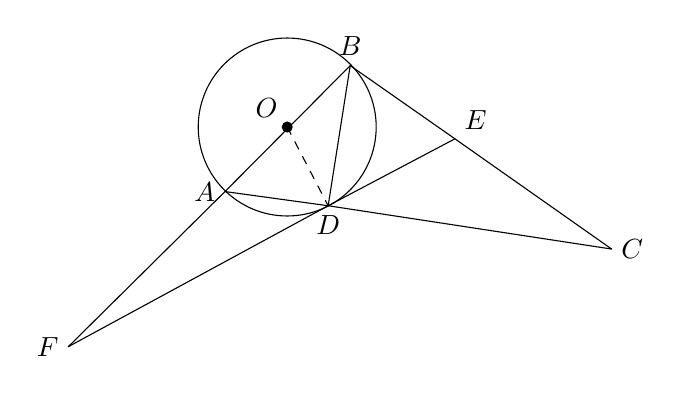
\begin{tikzpicture}[scale=1, line join=round, line cap=round]

\coordinate (O) at (3.45,-1.43);
\coordinate (B) at (4.25,-0.65);
\coordinate (A) at (2.66,-2.25);
\coordinate (D) at (3.97,-2.43);
\coordinate (E) at (5.58,-1.58);
\coordinate (C) at (7.57,-2.98);
\coordinate (F) at (0.67,-4.22);

\draw (O) circle (1.13);

\draw (F) -- (A) -- (B);
\draw (B) -- (E) -- (C);
\draw (A) -- (D) -- (C);
\draw (F) -- (D) -- (E);
\draw (B) -- (D);
\draw[dashed] (O) -- (D);

\fill (O) circle (2pt);

\node[above left] at (O) {$O$};
\node[above] at (B) {$B$};
\node[left] at (A) {$A$};
\node[below] at (D) {$D$};
\node[above right] at (E) {$E$};
\node[right] at (C) {$C$};
\node[left] at (F) {$F$};

\end{tikzpicture}
\end{document}
